\documentclass{article}
%%%%%%%%%%%%%%%%%
%%%%%%%%%%%%%%%%%%
\renewcommand{\thesubsection}{\thesection.\alph{subsection}}
\author{Matthew Bates}
\usepackage{xfrac}
\usepackage{amsmath}
\usepackage{fancyhdr}
\usepackage{gensymb}
\linespread{1.0}
\usepackage{graphicx}
\usepackage{subcaption}
\usepackage[font = footnotesize]{caption}
\usepackage{wrapfig}
\graphicspath{{C:/Users/C1764397/Workshop/DataMiningComp/Assignment2/}}
\usepackage[parfill]{parskip}
\usepackage{geometry}
\usepackage{hyperref}
\usepackage{breakcites}
\usepackage{listings}
%%%%%%%%%%%%%%%%%%%
\geometry{
a4paper,
total={150mm,237mm},
left = 30mm,
top = 30mm,
}
%%%%%%%%%%%%%%%%%%%
\hypersetup{
    colorlinks=false,
    pdfborder={0 0 0},
}
%%%%%%%%%%%%%%%%%%%
\pagestyle{fancy}
\lhead{Matthew Bates}
\chead{CMT108 - Pattern Recognition and Data Mining}
\rhead{Coursework II}
%%%%%%%%%%%%%%%%%%%
%%%%%%%%%%%%%%%%%%%

\begin{document}
\begin{titlepage}
    \begin{center}
        \vspace*{1cm}
        
	\Huge
        \textbf{Coursework II}
        
        \vspace{0.5cm}
	\LARGE
         \vfill

	CMT108 - Pattern Recognition and Data Mining\\
	Dr Padraig Corcoran\\
	School of Computer Science and Informatics\\
	Cardiff University\\
 	Wales, UK
        \vspace{1.5cm}

       	
\includegraphics[width=0.4\textwidth]{CardiffLogo.jpg}   
        
        \vspace{0.8cm}
        \Large
        \textbf{Matthew Bates - C1764397}\\
	PhD Student, Star Formation Group\\
        School of Physics and Astronomy\\
        Cardiff University\\
        Wales, UK\\
        27 April, 2018
        
    \end{center}
\end{titlepage}

\pagenumbering{arabic}

\section{Gradient Ascent}
\begin{figure}[h]
\centering
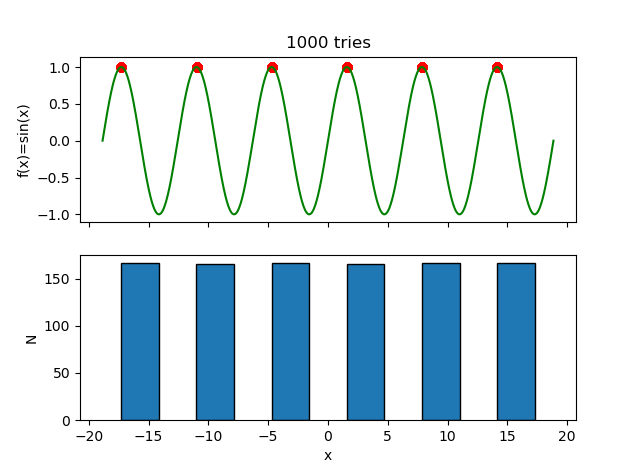
\includegraphics[width=0.9\linewidth]{Q1.png}
\caption{This figure shows the results of the gradient ascent function that is described in the text. Here we have randomly sampled 1000 initial guesses between $x=-6\pi$ and $x=6\pi$. The top graph shows the results of the gradient ascent (red) overlain over the function we are testing for (green). The bottom graph shows a distribution of the results, where it is pretty clear that it is uniform, which is as expected.}
\end{figure}

Given the following function, $f(x) = sin(x)$, we are asked to use a gradient ascent technique in order to find local maxima. The algorithm starts by choosing a random starting position, $x$, from a given range. The range used for this particular problem was from $x=-6\pi$ to $x=6\pi$. The initial guess is chosen from this range using a uniform random distribution. The gradient at this point, $m_x$ is then calculated. If $m_x >0$ then we assign $l=1$, if $m_x<0$ then $l=-1$. We then repeat this procedure for the point at $x_{new} = x+l\Delta x$. Here $\Delta x$ indicates the step size. We repeat this process until either $m_x\approx0$ or we have tried a number of points comparable to the number of points in the given range. The final point is the resulting local maximum.

Since the local maximum depends on our choice for initial guess then by choosing differing initial guesses we can find different local maxima. The algorithm was run 1000 times with each run choosing the initial guess from a uniform random distribution. This guarantees that we find all the local maxima within our range of interest. Plotting a distribution of the results shows that the local maxima are found with equal probability. See Figure 1.

The algorithm was written in Python 3 and is shown below:

\newpage

\noindent\rule{\textwidth}{1pt}
\begin{lstlisting}[language=Python]
import numpy as np
import matplotlib.pyplot as plt

#######################################################################
'''Functions'''
#######################################################################

def gradient_ascent(x,f,steps):

    df = np.gradient(f,x)
    
    initial_idx = np.random.randint(0,steps)
    next_idx = initial_idx
    
    conv = []
    
    for i in range(0,steps):
        
        if next_idx == steps:
            return np.nan
    
        grad = float(df[next_idx])
        
        if grad>0:
            step = 1
        elif grad<0:
            step = -1
        
        next_idx += step
        
        if i == steps-2:
            conv.append(next_idx)
        if i == steps-1:
            conv.append(next_idx)
        if abs(grad)<0.0001:
            return x[next_idx]
            
    conv = np.asarray(conv)    
    guess = []
    guess.append(x[conv[0]])
    guess.append(x[conv[1]])
    
    final_guess = np.mean(guess)
    
    return final_guess

#######################################################################
'''Implementation'''
#######################################################################

x = np.linspace(-6*np.pi,6*np.pi,1000)
f = np.sin(x)
steps = 1000

guesses = []

iterations = 1000

for k in range(0,iterations):
    guesses.append(gradient_ascent(x,f,steps))

guesses = np.asarray(guesses)
a,axarr = plt.subplots(2,sharex=True)
axarr[0].plot(x, f,c='g')
axarr[0].scatter(guesses,np.sin(guesses),c='r')
axarr[0].set_title('1000 tries')
axarr[0].set_ylabel('f(x)=sin(x)')
axarr[1].hist(x,bins = 6,rwidth = 0.5,edgecolor="k")
axarr[1].set_xlabel('x')
axarr[1].set_ylabel('N')
\end{lstlisting}
\noindent\rule{\textwidth}{1pt}

\newpage

\section{Student Probability}
\subsection{}
We are given that the probability of a student being a graduate student is $p(PG) = 0.3$. We are also given that students can either be graduate students or undergraduate students. Thus the probability of a student being an undergraduate student is,

\begin{equation}
p(UG) = 1 - p(PG) = 1 - 0.3 = 0.7
\end{equation}

Since $p(UG) > p(PG)$ we can safely say that a randomly selected student is more likely to be an undergraduate student.

\subsection{}
To find the probability that a female student is a graduate student, $p(PG|F)$, we use Bayes' rule:

\begin{equation}
p(PG|F) = \frac{p(F|PG)p(PG)}{p(F)}
\end{equation}

where
\begin{equation}
p(F) = p(F,PG)+p(F,UG) = p(F|PG)p(PG)+p(F|UG)p(UG)
\end{equation}

This gives
\begin{align}
p(PG|F) &= \frac{p(F|PG)p(PG)}{p(F|PG)p(PG)+p(F|UG)p(UG)}\\
&=\frac{0.33\times0.3}{(0.33\times0.3)+(0.25\times0.7)}\\
&=0.3613
\end{align}

Therefore the probability that a female student is a graduate student is $p(PG|F) = 0.3613$.

\subsection{}

\end{document}